\documentclass[paper=a4, fontsize=11pt]{scrartcl}
\usepackage{amsmath,amsfonts,amsthm}
\usepackage{sectsty}
\usepackage{fourier} % Use the Adobe Utopia font for the document - comment this line to return to the LaTeX default
\usepackage[english]{babel}
\allsectionsfont{ \normalfont\scshape}
\usepackage{fancyhdr}
\usepackage{float}
\usepackage{graphicx}
\usepackage{listings}
\pagestyle{fancyplain}

\fancyhead{} % No page header - if you want one, create it in the same way as the footers below
\fancyfoot[L]{} % Empty left footer
\fancyfoot[C]{} % Empty center footer
\fancyfoot[R]{\thepage} % Page numbering for right footer
\renewcommand{\headrulewidth}{0pt} % Remove header underlines
\renewcommand{\footrulewidth}{0pt} % Remove footer underlines
\renewcommand\floatpagefraction{.9}
\setlength{\headheight}{13.6pt} % Customize the height of the header
\numberwithin{equation}{section} % Number equations within sections (i.e. 1.1, 1.2, 2.1, 2.2 instead of 1, 2, 3, 4)
\numberwithin{figure}{section} % Number figures within sections (i.e. 1.1, 1.2, 2.1, 2.2 instead of 1, 2, 3, 4)
\numberwithin{table}{section} % Number tables within sections (i.e. 1.1, 1.2, 2.1, 2.2 instead of 1, 2, 3, 4)
\setlength\parindent{0pt} % Removes all indentation from paragraphs - comment this line for an assignment with lots of text
\renewcommand{\thesubsection}{\thesection\alph{subsection}}


\setlength\floatsep{1.25\baselineskip plus 2pt minus 2pt}
\setlength\textfloatsep{1.25\baselineskip plus 2pt minus 2pt}



%----------------------------------------------------------------------------------------
%	TITLE SECTION
%----------------------------------------------------------------------------------------

\newcommand{\horrule}[1]{\rule{\linewidth}{#1}} % Create horizontal rule command with 1 argument of height
\title{	
\normalfont \normalsize 
\textsc{Yale-NUS College} \\ [20pt]
\textsc{YID3202C : Data Analysis in Environmental Studies } \\ [25pt] % Your university, school and/or department name(s)
\horrule{0.5pt} \\[0.4cm] % Thin top horizontal rule
\huge Problem Set Four \\ % The assignment title
\horrule{2pt} \\[0.5cm] % Thick bottom horizontal rule
}

\author{Jake Goh Si Yuan} % Your name

\date{\normalsize October 24, 2016} % Today's date or a custom date


\begin{document}

\maketitle % Print the title
\section{Computations Associated With the Discrete Fourier Transform}
\subsection{}
Let us simplify our lives here and start with some identities.

\begin{align*}
-i2\pi f_{+} n \Delta t &= -i2\pi (f_N + \tilde{f})n\Delta t & -i2\pi f_{-} n \Delta t &= -i2\pi (f_N - \tilde{f})n\Delta t \\
&= -i2n\Delta t\pi (f_N + \tilde{f}) &  &=-i2\pi n\Delta t (f_N - \tilde{f}) \\
&= -in\pi -i2n\Delta t\pi \tilde{f} &  &=-in\pi  +i2\pi n\Delta t \tilde{f} \\
\end{align*}

From this, we can first look at the exponent part of the expressions, using Euler's formula to arrive at the trignometric equivalents.
First, let $k = 2n\Delta t \pi$.
\begin{align*}
\exp(-in\pi -ik\tilde{f}) &= \exp(-in\pi) \exp(-ik\tilde{f}) & \exp(-in\pi +ik\tilde{f}) &= \exp(-in\pi) \exp(ik\tilde{f}) \\
&= (-1)^n(\cos(ik\tilde{f}) - i\sin(ik\tilde{f})) & &= (-1)^n(\cos(ik\tilde{f}) + i\sin(ik\tilde{f}))
\end{align*}

Factoring in the $Z$ and $Z^*$.
\begin{align*}
Z(-1)^n(\cos(ik\tilde{f}) - i\sin(ik\tilde{f})) &= (A+iB) (-1)^n(\cos(ik\tilde{f}) - i\sin(ik\tilde{f})) \\ 
Z^*(-1)^n(\cos(ik\tilde{f}) + i\sin(ik\tilde{f})) &= (A-iB) (-1)^n(\cos(ik\tilde{f}) + i\sin(ik\tilde{f}))
\end{align*}

Taking only real parts:
\begin{align*}
\mathbb{R}((A+iB) (-1)^n(\cos(ik\tilde{f}) - i\sin(ik\tilde{f}))) &= (-1)^n(A\cos(ik\tilde{f})+B\sin(ik\tilde{f}))\\
\mathbb{R}((A-iB) (-1)^n(\cos(ik\tilde{f}) + i\sin(ik\tilde{f}))) &= (-1)^n(A\cos(ik\tilde{f})+B\sin(ik\tilde{f}))
\end{align*}

As we can see, the expressions end up to be the same, thus a cyclic signal with frequency $f_+$ will alias into frequency of $f_-$.
\subsection{}

To begin the question, let us look at the exponents itself again.
\begin{align*}
\exp(+i2\pi f_p n\Delta t) \exp(-i2\pi f_q n\Delta t) &= \exp(i2\pi f_p n\Delta t -i2\pi f_q n\Delta t) \\
&= \exp(i2\pi n\Delta t (f_p - f_q))
\end{align*}

Since $f_p = \frac{p}{N\Delta t}$ and $f_q = \frac{q}{N\Delta t}$,
$$\exp(i2\pi n\Delta t (\frac{p-q}{N\Delta t})) = \exp(i2\pi n (\frac{p-q}{N}))$$

Now let us take a look at the equation.
\begin{align*}
\sum^{N-1}_{n=0}\exp(+i2\pi f_p n\Delta t) \exp(-i2\pi f_q n\Delta t) &= \sum^{N-1}_{n=0}\exp(i2\pi n (\frac{p-q}{N}))\\
&= \frac{1-\exp(i2\pi (p-q))}{1-\exp(i2\pi\frac{p-q}{N})} \\
\end{align*}

When $p \neq q$, the numerator is zero while the denominator is non-zero, which proves that the vectors are mutually orthogonal according to the formula.


\section{The Dirichlet Kernel}

\subsection{}
\begin{figure}[htp]
	\centering
	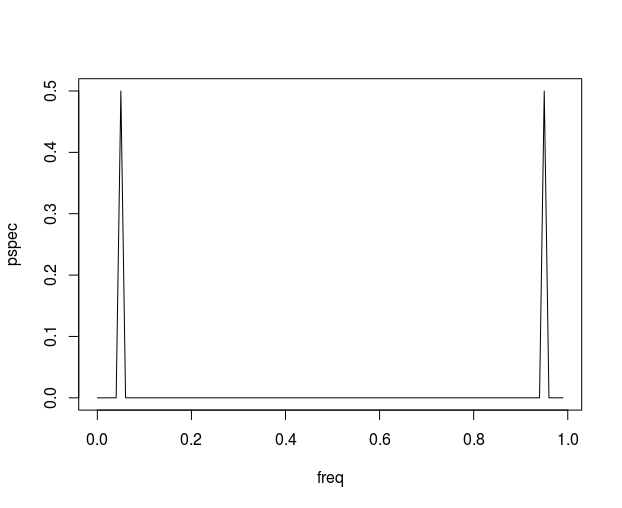
\includegraphics[width=0.7\textwidth, clip]{q1aa.png} 
	\caption{Absolute valued part of FFT}
\end{figure}

\begin{figure}[htp]
	\centering
	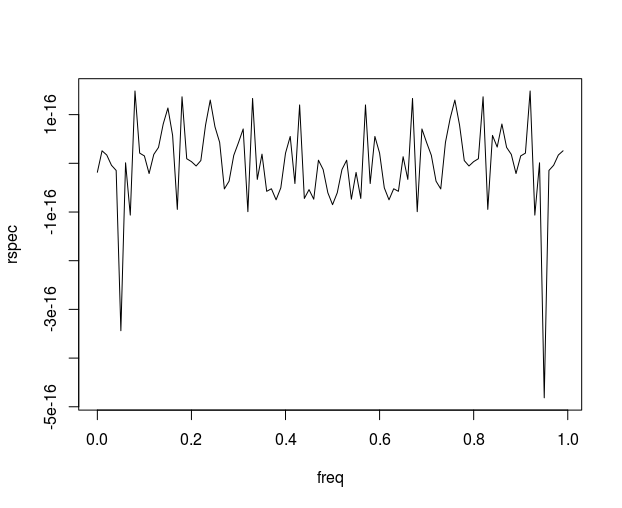
\includegraphics[width=0.7\textwidth, clip]{q1ab.png} 
	\caption{Real part of FFT}
\end{figure}
\pagebreak
\begin{figure}[htp]
	\centering
	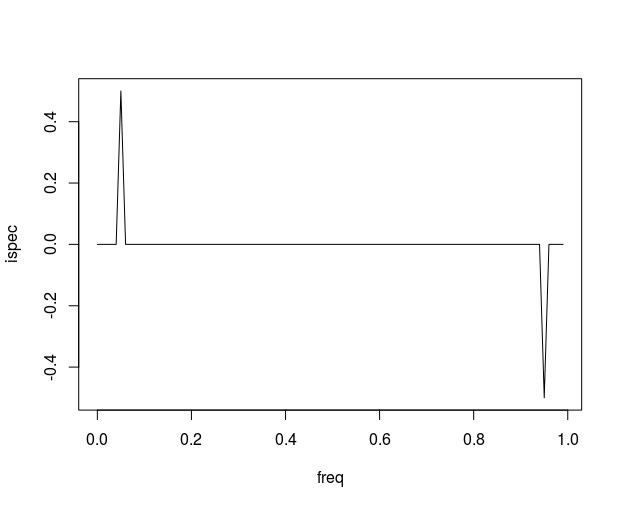
\includegraphics[width=0.7\textwidth, clip]{q1ac.png} 
	\caption{Imaginary part of FFT}
\end{figure}

The absolute part of the raw DFT is the Pythagorean sum of the imaginary and real parts of the DFT. Although it is not immediately clear from the graphs, we can take reference from the absolute value spikes at approximately 0.02 and 0.09, corresponding that with the spikes on the Imaginary value graph, and the 'anti'-spike on the Real graph. 

The Real part of the DFT appears to carry relative-to-itself significant value when the Imaginary part is relative-to-itself insignificant.

\subsection{}
\begin{figure}[htp]
	\centering
	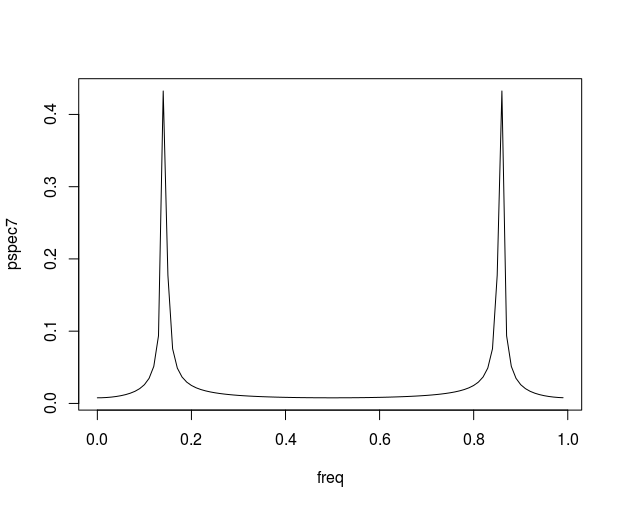
\includegraphics[width=0.7\textwidth, clip]{q1ba.png} 
	\caption{Absolute valued part of FFT}
\end{figure}

\begin{figure}[htp]
	\centering
	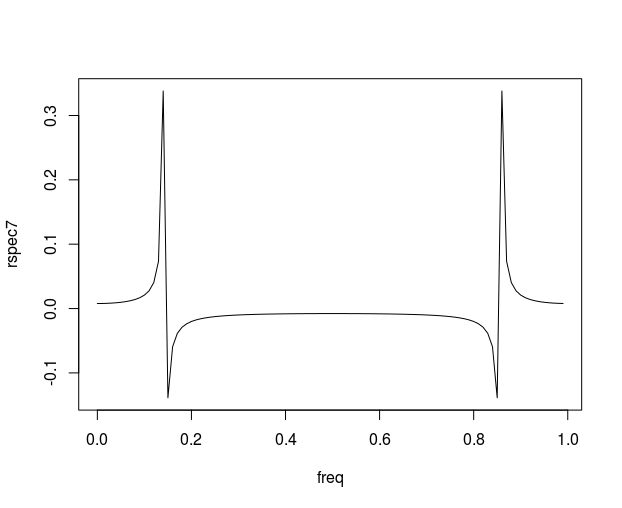
\includegraphics[width=0.7\textwidth, clip]{q1bb.png} 
	\caption{Real part of FFT}
\end{figure}
\pagebreak
\begin{figure}[htp]
	\centering
	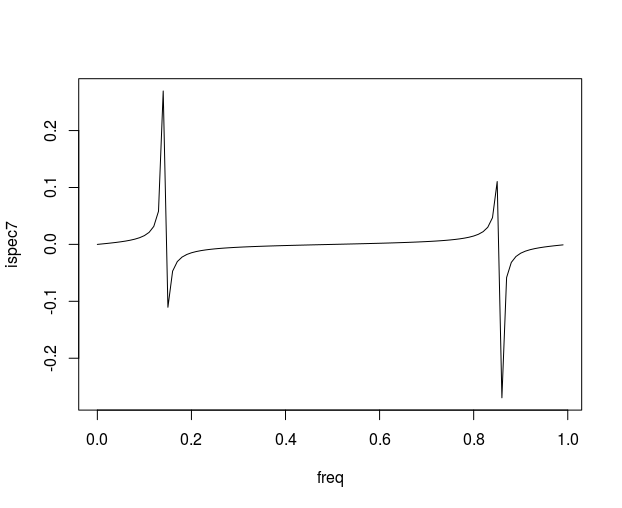
\includegraphics[width=0.7\textwidth, clip]{q1bc.png} 
	\caption{Imaginary part of FFT}
\end{figure}

The spikes at the absolute valued part appears to be better related now with the real and imaginary part, with the latter two graphs receiving a similar change in activity at approximately the same positions. The real and imaginary parts also carry a more similar characteristic in terms of the shape of the graph, although it has to be noted that for the higher frequency spike, the imaginary part of the DFT is slightly distorted with a lower-tending spike, whilst the real part of the DFT keeps a symmetrical shape, much like the absolute valued part.
\pagebreak
\subsection{}
\begin{figure}[htp]
	\centering
	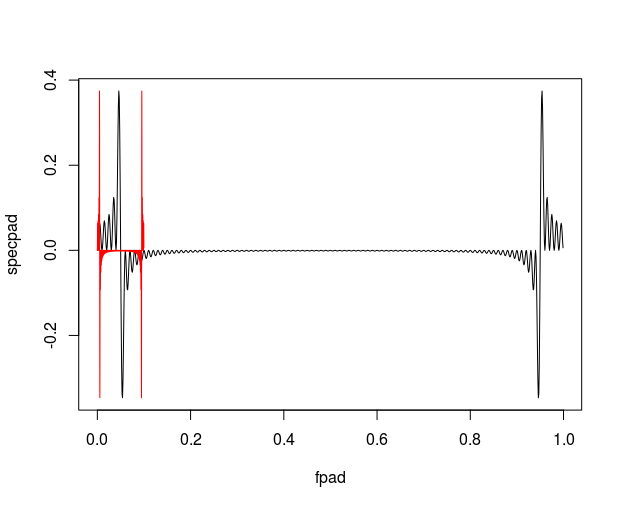
\includegraphics[width=0.7\textwidth, clip]{q1c.png} 
	\caption{FFT with padding, with $0\leq$fpad$<0.1$ in red}
\end{figure}

With the extra padding of 900 zeroes, the FFT takes on a more familiar Fourier transform shape.
The general shape takes on the spikes at the two positions as we have discussed in the previous two parts, with a much more gradual build up towards it, and a gradual flattening in between them. The part in between them where not much value is expected are better expressed of their true characteristic as opposed to the pseudo flat lines from before.

The portion of $0\leq$fpad$<0.1$ occupies the space as defined, with the same shape of the bigger graph compressed into the range.
\pagebreak
\section{Statistics of the Peridogram}
\subsection{}

\begin{figure}[htp]
	\centering
	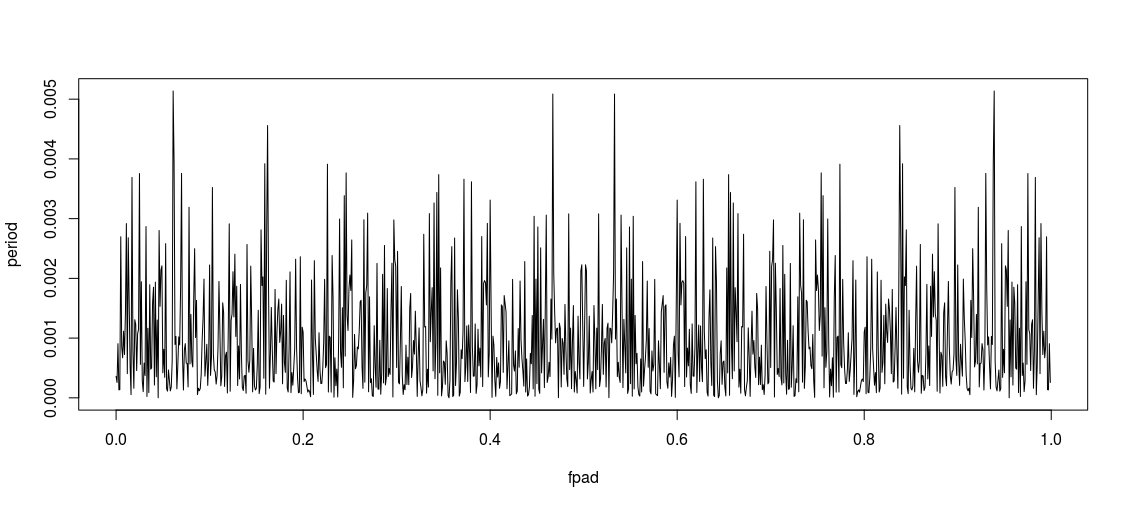
\includegraphics[width=0.7\textwidth, clip]{q3a.png} 
	\caption{Absolute value squared of FFT of 1000 Gaussian~N(0,1) sampled values}
\end{figure}

The expectation value is 0.001001572.
\pagebreak
\subsection{}
\begin{figure}[htp]
	\centering
	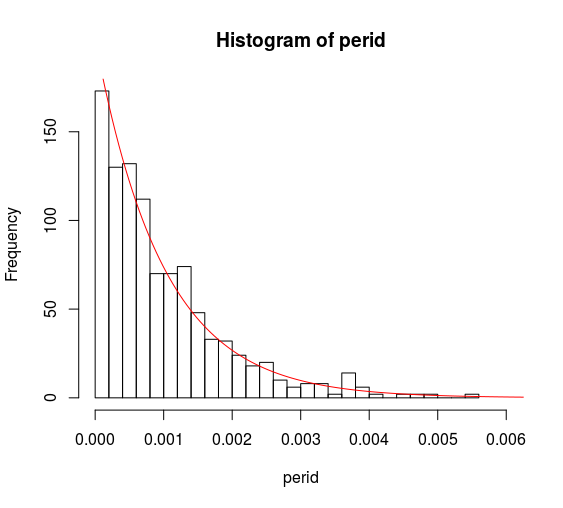
\includegraphics[width=0.7\textwidth, clip]{q3b.png} 
	\caption{Histogram of absolute value squared of FFT of 1000 Gaussian~N(0,1) sampled values overlayed with chi-squared PDF in red}
\end{figure}

The theory seems to hold very well here as the chi-squared model fits the histogram for the peridogram relatively well.
\end{document}